% Paper order changed back. The original order first etsablished thrmbolysis works as expected, then goes on to analyse who is receiving it. So paper 3 (clinical trial) supoports paper 4 (rather than vice versa).

\section{Paper 3 highlights: Thrombolysis: Are the results from the clinical trial meta-analysis seen in real life outcomes?  A machine learning study of the UK stroke registry.\cite{pearn_thrombolysis_2024}}\label{sec:paper_3}

\subsection{Objective}

To investigate, using explainable machine learning, the benefit of thrombolysis, and to compare the relationship between time-to-treatment and effectiveness with clinical trial results.

\subsection{Methods overview}

Data for a total of 168,347 ischaemic stroke patients who attended one of 118 emergency stroke hospitals in England and Wales from 2016 to 2021 were extracted from the Sentinel Stroke National Audit Programme (SSNAP). We used explainable machine learning (XGBoost\cite{chen_xgboost_2016} with SHAP\cite{lundberg_unified_2017}) to examine the effect of patient characteristics, hospital attended, and use/time of thrombolysis on the odds of achieving a good outcome (being at or below any given modified Rankin Scale threshold). A linear regression model was fitted to the estimated effect of onset-to-treatment time on thrombolysis to permit comparison with clinical trial meta-analyses.

Code, and full results, for the machine learning work may be found at \url{https://github.com/samuel-book/thrombolysis_clinical_trials_ml_paper}

\subsection{Key results}

\subsubsection{Feature selection}

Using the results from Pearn \textit{el at}. \cite{pearn_are_2024}, we selected seven features as inputs for the model to predict a patient's likelihood of a good outcome at discharge:

\begin{enumerate}
    % No need for saying coding of Yes/No is 1/0
    \item Prior disability level: Estimated mRS score prior to stroke
    \item Stroke severity: National Institutes of Health Stroke Scale (NIHSS) score on arrival
    \item Stroke team: Stroke team attended (hospital identifier)
    \item Age: Age (as midpoint of 5 year age bands)
    \item Onset to thrombolysis time: Time from onset to receiving thrombolysis (minutes). This was set to 9999 if the patient did not receive thrombolysis.
    \item Atrial fibrillation diagnosis: Patient had a diagnosis of atrial fibrillation, either on arrival or diagnosed during admission
    \item Precise onset time known: Onset time recorded was recorded as being precise time, as opposed to a best estimate (\textit{precise} or  \textit{best estimate})
\end{enumerate}

Code and full results for feature selection may be found at \url{https://github.com/samuel-book/feature_selection_thrombolysis_outcome_ml_paper}

\subsubsection{Model accuracy}

With 7 input features, overall accuracy ranged from 77.6\% to 89.7\% across the six models (standard deviation across the 5 k-folds ranged from 0.001 to 0.002). This represented between 95-98\% of the accuracy that is obtained with all the features as inputs. Receiver Operating Characteristic Area Under Curve (ROC-AUC) ranged from 0.852 to 0.893 across the six models (standard deviation across the 5 k-folds ranged from 0.001 to 0.002).

\subsubsection{Global SHAP patterns}

SHAP values explain the contribution (as the change in log-odds) that each feature value has on the model’s prediction of achieving a good outcome at discharge \cite{lundberg_unified_2017}. SHAP values expressed as log-odds are additive (and so are preferred to probabilities, which are not additive, when examining the contribution of individual features to the final prediction). A SHAP model for each of the six machine learning models was created (one for each threshold of mRS to define a good outcome). To illustrate how to interpret the SHAP value in our case, the target feature with a value of 1 represents a good outcome (being at or below any given mRS threshold), and a value 0 represents a worse outcome (being above any given mRS threshold). A positive SHAP value represents that the corresponding feature value increases the likelihood for that patient having a good outcome, and a negative SHAP value represents that the corresponding feature value reduces the likelihood for that patient having a good outcome. SHAP values can be assessed \textit{locally} at patient level, and \textit{globally} at patient cohort level to understand general patterns of how discharge outcomes differ by each of the patient, pathway, and hospital characteristics.

For each patient in the test set we extracted SHAP values for each feature with its corresponding feature value. Figure \ref{fig:global_shap_mrs1} shows the relationship between feature values and the odds of a patient having a good outcome (mRS 0-1) at discharge (a positive SHAP value contributes to an increased likelihood, and a negative SHAP value contributes to a reduced likelihood). We see that low prior disability, lower stroke severity, younger age, receiving thrombolysis (and receiving it sooner after onset), and having no diagnosis of atrial fibrillation contributed to a patient more likely having a good outcome at discharge. Figure \ref{fig:global_shap_ott} focusses on the feature \textit{onset to thrombolysis time}, and its effect at reaching any disability threshold. As time from onset to treatment increased, the beneficial effect of thrombolysis decayed. For thresholds up to, and including, mRS 3, the median effect of thrombolysis remained positive, compared to not receiving thrombolysis, up until the maximum time of 720 minutes. For thresholds of mRS 4 and upwards, the median effect of thrombolysis became negative at longer onset-to-treatment times. This was especially apparent in how thrombolysis changed the overall odds of survival (mRS 0-5) where the median effect of thrombolysis became negative from about 155 minutes. Later thrombolysis may therefore increase the proportion of patients attaining mRS 0-3, but at the cost of some reduction in overall survival. Earlier thrombolysis improved the odds of survival. Figure \ref{fig:global_shap_hosp} shows the contribution from attending a specific hospital to predicting whether the patient had a good outcome at discharge, for each of the mRS threshold levels used to define a good outcome. As the threshold for having a good outcome becomes more inclusive, the range of the effect of the hospital attended had a reduced contribution on the prediction.


\begin{sidewaysfigure}[!h]
    \centering
    \begin{subfigure}[b]{0.8\textwidth}
      \centering
      
\includegraphics[trim={0 0 0 1.2cm}, clip, width=1\textwidth]{./images/p3_clin_shap_sub_1}\\
      \caption{The relationship between feature values and the prediction of whether a patient will have a good outcome (mRS 0-1) at discharge. SHAP base value for this model is -1.529.}
      \label{fig:global_shap_mrs1}
    \end{subfigure}
    \hfill
    \begin{subfigure}[b]{0.8\textwidth}
      \centering    
      
\includegraphics[width=1\textwidth]{./images/p3_clin_shap_sub_2.jpg}\\
%      \includegraphics[trim={0 0 0 1.2cm}, clip, width=1\textwidth]{./images/083_xgb_7_features_5fold_binary_shap_violin_ss_0kfold}\\
      \caption{The relationship between onset to thrombolysis time and the prediction of whether a patient will have a good outcome at discharge, for each of the mRS scores used to define a good outcome.}
      \label{fig:global_shap_ott}
    \end{subfigure}
    \hfill
    \begin{subfigure}[b]{0.8\textwidth}
      \centering
      
\includegraphics[trim={0 0 0 1.2cm}, clip, width=1\textwidth]{./images/p3_clin_shap_sub_3}\\
      \caption{The contribution from attending a specific hospital to predicting whether the patient will have a good outcome at discharge, for each of the mRS scores used to define a good outcome}
      \label{fig:global_shap_hosp}
    \end{subfigure}
    \label{fig:global_shap_trio}
  \caption{The relationship between feature values SHAP values in predicting whether a patient will have a good outcome. Violin plots show the distribution of SHAP values across the patient population for each feature value, with the mid-line showing the median SHAP value.} 
\end{sidewaysfigure}

%\FloatBarrier


\subsubsection{The direct contribution of thrombolysis use to the shift in probability of a good outcome}

We used the first k-fold train/test set split (4:1 train:test data) to investigate likely outcome from thrombolysis. For each patient in the test set that received thrombolysis within 300 minutes from stroke onset (n = 6,796), we performed a counterfactual analysis, predicting outcome probabilities if the patient had not received thrombolysis. We calculated the effect of thrombolysis by taking the difference in SHAP values, between treated and the predicted outcome if untreated, for the contribution of thrombolysis to achieving a good outcome.

We modelled the decay in effect of thrombolysis by fitting a linear regression model to the benefit of thrombolysis (log odds shift in attaining a good outcome) with time from onset to treatment (excluding patients treated after 300 minutes). The model used the definition of mRS 0-1 as a good outcome to match the definition used in the meta-analysis of clinical trials \cite{emberson_effect_2014}. The analysis was applied to three patient cohorts: (1) all treated ischaemic strokes (n = 6,796), (2) treated severe ischaemic strokes, NIHSS 11+ (n = 2,856), (3) treated mild-moderate ischaemic strokes, NIHSS 0-10 (n = 3,940). 

Figure \ref{fig:linear_regression_plots} shows a linear regression fitted to the shift in the contribution from receiving thrombolysis towards having a good outcome at discharge (mRS 0-1) with respect to the onset to thrombolysis time. We found, for all treated patients, that the effect of thrombolysis had declined to zero at 328 minutes, and the effect from thrombolysis was improving log odds of a good outcome by 0.90 if it were, theoretically, given at the time of stroke onset. We observed that the maximum theoretical effect of thrombolysis (if given at time of stroke onset) was greater for the severe stroke group (1.048 log odds) than the mild-moderate stroke group (0.771 log odds). However the effect of thrombolysis declined a little faster in the severe stroke group (reaching no effect at 314 minutes for severe stroke patients, compared to 351 minutes for mild-moderate stroke patients). Linear regression coefficients in all three patient groups were statistically significant (table \ref{fig:stats_table_mrs1}). 

\begin{figure}
    \centering
    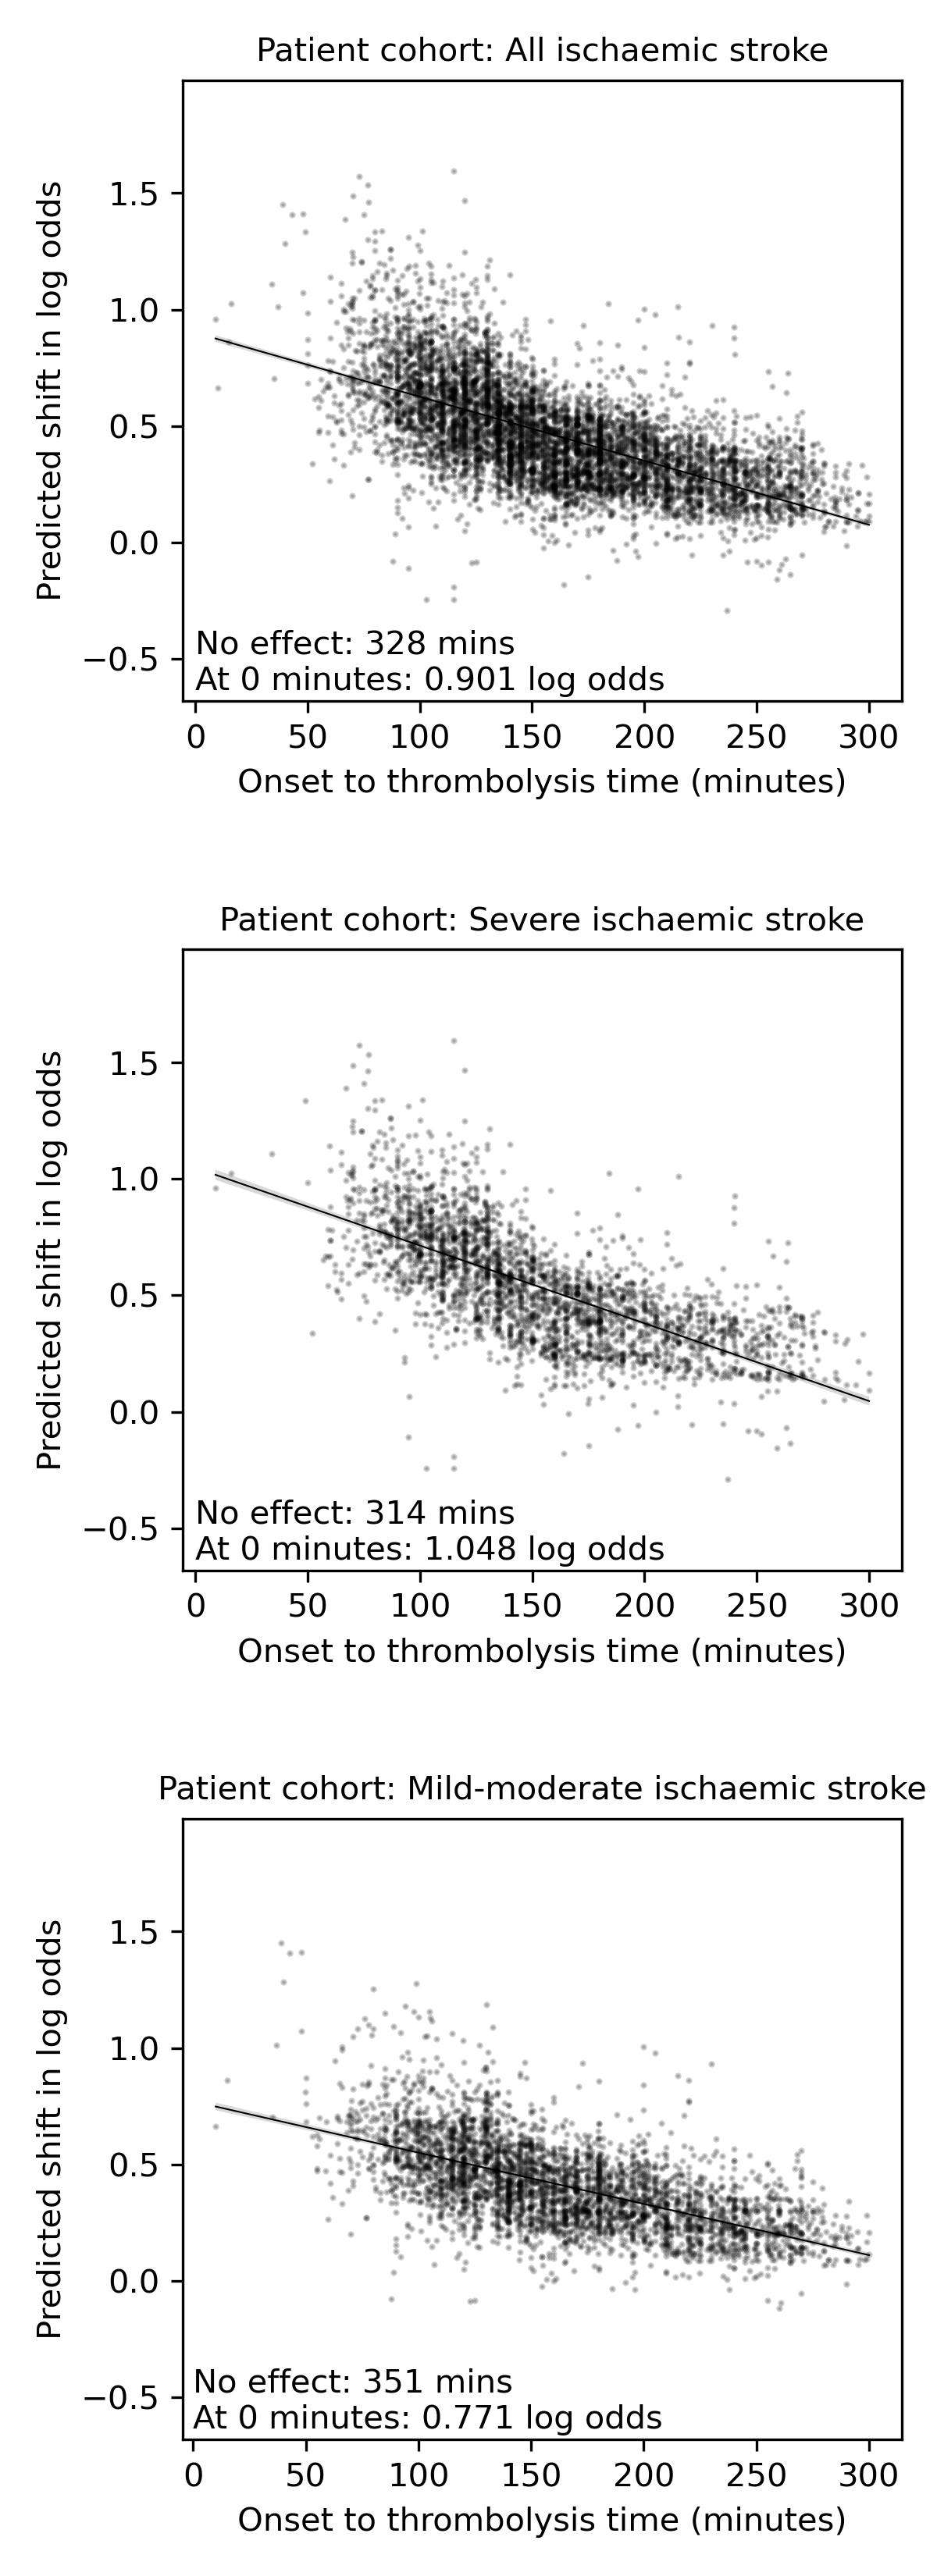
\includegraphics[width=0.40\textwidth]{./images/p3_regression_v1}\\
    \caption{A linear regression fit to the contribution from receiving thrombolysis in having a good outcome (mRS 0-1) at discharge, with respect to the onset to thrombolysis time (for patients treated within 300 minutes). Top: all treated stroke patients (n = 6,796); Middle: treated severe stroke patients, NIHSS 11+ (n = 2,856); Bottom: treated mild-moderate stroke patients, NIHSS 0-10 (n = 3,940).}
    \label{fig:linear_regression_plots}
\end{figure}

\begin{table}
    \caption{Fitting linear regression to the shift in the contribution from receiving thrombolysis towards having a good outcome (mRS 0-1) at discharge with respect to the onset to thrombolysis (OTT) time. Linear regression statistics for different patient cohorts. We used NIHSS 0-10 to define mild-moderate strokes, and NIHSS 11+ to define severe strokes.}
    \centering
        \begin{tabular}{lllllllll}
        \toprule
         Ischaemic stroke type & Variables & coef & std err & t & P$>$$|$t$|$ & [0.025 & 0.975] \\ 
         \midrule
        All & Constant & 0.9012 & 0.007 & 132.519 & 0.000 & 0.888 & 0.915\\
        & OTT time (min) &  -0.0027  & 4.04e-05 & -68.058 & 0.000 & -0.003 & -0.003\\   
        \midrule
        Severe & Constant & 1.0476  &    0.011  & 96.746 & 0.000 & 1.026 & 1.069\\
        & OTT (mins) & -0.0033 &  6.67e-05  & -50.042 & 0.000 & -0.003 & -0.003\\ 
        \midrule
        Mild-moderate & Constant &           0.7708 &     0.008   & 97.613 & 0.000 & 0.755 & 0.786\\
        & OTT time (mins) &  -0.0022 &   4.57e-05 & -48.109 & 0.000 & -0.002 & -0.002\\
        \bottomrule
        \end{tabular}
      \label{fig:stats_table_mrs1}
\end{table}

\subsection{Conclusions}

Using machine learning methods with SHAP in a very large prospective national stroke registry, thrombolysis was found to be associated with a statistically significant improvement in the odds of having a good outcome using any mRS threshold. Regression analysis predicted a maximum 2.5-fold improvement in odds of achieving mRS 0-1, with a decline to no treatment effect at 5 hours 28 minutes post-onset. The findings from this study were remarkably similar to the meta-analysis of clinical trials 8, which extrapolate back to a 0.69 log odds (equivalent to an odds ratio of 2.0) improvement of being mRS 0-1 at stroke onset, with no effect after 6 hours 18 minutes.